%%%%%%%%%%%%%%%%%%%%%%%%%%%%%%%%%%%%
% Slide options
%%%%%%%%%%%%%%%%%%%%%%%%%%%%%%%%%%%%

% Option 1: Slides with solutions

\documentclass[slidestop,compress,mathserif]{beamer}
\usepackage{booktabs}
\newcommand{\soln}[1]{\textit{#1}}
\newcommand{\solnGr}[1]{#1}

% Option 2: Handouts without solutions

%\documentclass[11pt,containsverbatim,handout]{beamer}
%\usepackage{pgfpages}
%\pgfpagesuselayout{4 on 1}[letterpaper,landscape,border shrink=5mm]
%\newcommand{\soln}[1]{ }
%\newcommand{\solnGr}{ }

%%%%%%%%%%%%%%%%%%%%%%%%%%%%%%%%%%%%
% Style
%%%%%%%%%%%%%%%%%%%%%%%%%%%%%%%%%%%%
%%%%%%%%%%%%%%%%%%%%%%%%%%%%%%%%%%%%%%%%%%%%%%%%%%%%%%%%%%%%%%%%%%%%%%%%
% MA213/214 shared slide style
%
% "Calm & Cool" palette + content-type callout boxes.
% Overhauled (2026) from the original OpenIntro/metropolis style:
%   - all OpenIntro visual branding removed (logo, grid, colors)
%   - a low-key cool palette (see colors below)
%   - tcolorbox callout boxes so students recognize content types
% See common/README.md for the command cheat-sheet.
%%%%%%%%%%%%%%%%%%%%%%%%%%%%%%%%%%%%%%%%%%%%%%%%%%%%%%%%%%%%%%%%%%%%%%%%

\usetheme{metropolis}

%%%%%%%%%%%%%%%%
% Packages
%%%%%%%%%%%%%%%%

\usepackage{geometry}
\usepackage{graphicx}
\usepackage{amssymb}
\usepackage{epstopdf}
\usepackage{amsmath}  	% this permits text in eqnarray among other benefits
\usepackage{url}		% produces hyperlinks
\usepackage{hyperref}	% allows for color usage in tables
\usepackage[english]{babel}
\usepackage[latin1]{inputenc}
\usepackage{colortbl}	% allows for color usage in tables
\usepackage{multirow}	% allows for rows that span multiple rows in tables
\usepackage{color}		% this package has a variety of color options
\usepackage{pgf}
\usepackage{calc}
\usepackage{ulem}
\usepackage{multicol}
\usepackage{textcomp}
\usepackage{txfonts}
\usepackage{listings}
\usepackage{tikz}
\usepackage{array}
\usepackage{wasysym}
\usepackage{fancyvrb}
\usepackage{etoolbox}             % \ifstrempty for optional box subtitles
\usepackage[most]{tcolorbox}      % content-type callout boxes
\tcbuselibrary{listings}          % R-code block (\begin{rblock})
\usepackage{fontawesome5}         % box icons

%%%%%%%%%%%%%%%%
% Remove navigation symbols
%%%%%%%%%%%%%%%%

\setbeamertemplate{navigation symbols}{}

%%%%%%%%%%%%%%%%
% "Calm & Cool" palette
%%%%%%%%%%%%%%%%

% chrome / structure / body
\definecolor{ccSlate}{HTML}{2E3742}   % frametitle bar, structure, section pages (deep neutral slate)
\definecolor{ccInk}{HTML}{2B2B2B}     % body text
\definecolor{ccWash}{HTML}{FCF8F1}    % gentle warm title-slide background wash (complements the cool blues)

% example (blue)
\definecolor{ccBlue}{HTML}{2F6690}
\definecolor{ccBlueBg}{HTML}{EAF1F7}
% interactive activity / discussion (green)
\definecolor{ccGreen}{HTML}{4E8A6B}
\definecolor{ccGreenBg}{HTML}{E9F3EC}
% solution (purple)
\definecolor{ccPurple}{HTML}{6F5499}
\definecolor{ccPurpleBg}{HTML}{EFEAF6}
% worksheet / focused work (terracotta)
\definecolor{ccTerra}{HTML}{C2693E}
\definecolor{ccTerraBg}{HTML}{FAEDE4}
% formula / definition (neutral slate)
\definecolor{ccGray}{HTML}{5C6B7A}
\definecolor{ccGrayBg}{HTML}{EEF1F4}
% caution / common pitfall (brick red)
\definecolor{ccRed}{HTML}{B23A48}
\definecolor{ccRedBg}{HTML}{FAEAEC}
% key idea / takeaway (muted gold)
\definecolor{ccGold}{HTML}{9C7A28}
\definecolor{ccGoldBg}{HTML}{F7F1DF}
% learning goals / lesson outcomes (teal)
\definecolor{ccTeal}{HTML}{2C6E6B}
\definecolor{ccTealBg}{HTML}{E6F0EF}
% learning objectives (indigo)
\definecolor{ccIndigo}{HTML}{45507A}
\definecolor{ccIndigoBg}{HTML}{ECEEF4}
% R code / output (gray)
\definecolor{ccCode}{HTML}{5F5E5A}
\definecolor{ccCodeBg}{HTML}{F4F5F6}

% neutral grays kept from the original style
\definecolor{gray}{rgb}{0.5, 0.5, 0.5}
\definecolor{darkGray}{rgb}{0.3, 0.3, 0.3}
\definecolor{darkerGray}{rgb}{0.2, 0.2, 0.2}

% Backwards-compatible aliases: old OpenIntro color names now point at the
% new palette, so existing \textcolor{oiB}{...}, \hl{...}, etc. keep working.
\colorlet{oiB}{ccBlue}
\colorlet{oiG}{ccGreen}
\colorlet{hlblue}{ccBlue}
\colorlet{rubineRed}{ccRed}
\colorlet{irishGreen}{ccGreen}
\colorlet{lightGreen}{ccGreen}

%%%%%%%%%%%%%%%%
% Restyle metropolis with the Calm & Cool chrome
%%%%%%%%%%%%%%%%

\metroset{block=fill}

\setbeamercolor{normal text}{fg=ccInk, bg=white}
\setbeamercolor{structure}{fg=ccSlate}
\setbeamercolor{alerted text}{fg=ccBlue}
\setbeamercolor{example text}{fg=ccGreen}
\setbeamercolor{frametitle}{bg=ccSlate, fg=white}
\setbeamercolor{progress bar}{fg=ccBlue}
\setbeamercolor{title separator}{fg=ccBlue}
\setbeamercolor{title}{fg=ccSlate}
\setbeamercolor{subtitle}{fg=ccBlue}
\setbeamercolor{author}{fg=ccInk}
\setbeamercolor{institute}{fg=ccGray}
\setbeamercolor{date}{fg=ccGray}
\setbeamercolor{section title}{fg=ccSlate}
\setbeamercolor{standout}{fg=white, bg=ccSlate}

% Section pages sit on the same warm wash as the title slide. We keep
% metropolis's section-title styling and just paint a full-page ccWash
% background behind it (needs >=2 pdflatex passes for the current-page node).
\setbeamertemplate{section page}{%
  \begin{tikzpicture}[remember picture, overlay]
    \fill[ccWash] (current page.south west) rectangle (current page.north east);
  \end{tikzpicture}%
  \centering
  \begin{minipage}{22em}
    \raggedright
    \usebeamercolor[fg]{section title}%
    \usebeamerfont{section title}%
    \insertsectionhead\\[-1ex]
    \usebeamertemplate*{progress bar in section page}%
    \par
  \end{minipage}\par
  \vspace{\baselineskip}
}

%%%%%%%%%%%%%%%%
% Custom inline text commands (recolored to the palette)
%%%%%%%%%%%%%%%%

% degree
\newcommand{\degree}{\ensuremath{^\circ}}

% cite
\newcommand{\ct}[1]{
\vfill
{\tiny #1}}

\newcommand{\NamedNote}[2]{
\rule{2.5cm}{0.25pt} \\ \textit{\footnotesize{\textcolor{rubineRed}{#1:} \textcolor{darkerGray}{#2}}}}

% Note
\newcommand{\Note}[1]{
\rule{2.5cm}{0.25pt} \\ \textit{\footnotesize{\textcolor{rubineRed}{Note:} \textcolor{darkerGray}{#1}}}}

% Remember
\newcommand{\Remember}[1]{\textit{\scriptsize{\textcolor{ccTerra}{Remember:} #1}}}

% expected counts
\newcommand{\ex}[1]{\textit{\textcolor{ccBlue}{#1}}}

% red
\newcommand{\red}[1]{\textit{\textcolor{rubineRed}{#1}}}

% pink
\newcommand{\pink}[1]{\textit{\textcolor{rubineRed!90!white!50}{#1}}}

% green
\newcommand{\green}[1]{\textit{\textcolor{irishGreen}{#1}}}

% orange
\newcommand{\orange}[1]{\textit{\textcolor{ccTerra}{#1}}}

% links: webURL, webLink, appLink
\newcommand{\webURL}[1]{\urlstyle{same}{ \textit{\textcolor{darkGray}{\url{#1}}}}}
\newcommand{\webLink}[2]{\href{#1}{\textcolor{darkGray}{{#2}}}}
\newcommand{\appLink}[2]{\href{#1}{\textcolor{white}{{#2}}}}

% mail
\newcommand{\mail}[1]{\href{mailto:#1}{\textit{\textcolor{darkGray}{#1}}}}

% highlighting: hl, hlGr, mathhl
\newcommand{\hl}[1]{\textit{\textcolor{hlblue}{#1}}}
\newcommand{\hlGr}[1]{\textit{\textcolor{lightGreen}{#1}}}
\newcommand{\mathhl}[1]{\textcolor{hlblue}{\ensuremath{#1}}}

%%%%%%%%%%%%%%%%
% Structural helpers (unchanged from the original)
%%%%%%%%%%%%%%%%

% two col: two columns
\newenvironment{twocol}[4]{
\begin{columns}[c]
\column{#1\textwidth}
#3
\column{#2\textwidth}
#4
\end{columns}
}

% slot (for probability calculations)
\newenvironment{slot}[2]{
\begin{array}{c}
\underline{#1} \\
#2
\end{array}
}

% pr: left and right parentheses
\newcommand{\pr}[1]{
\left( #1 \right)
}

% cancel
\newcommand{\cancel}[1]{%
    \tikz[baseline=(tocancel.base)]{
        \node[inner sep=0pt,outer sep=0pt] (tocancel) {#1};
        \draw[red, line width=0.5mm] (tocancel.south west) -- (tocancel.north east);
    }%
}

% removepagenumbers
\newcommand{\removepagenumbers}{%
  \setbeamertemplate{footline}{}
}

% change margin
\newenvironment{changemargin}[2]{%
\begin{list}{}{%
\setlength{\topsep}{0pt}%
\setlength{\leftmargin}{#1}%
\setlength{\rightmargin}{#2}%
\setlength{\listparindent}{\parindent}%
\setlength{\itemindent}{\parindent}%
\setlength{\parsep}{\parskip}%
}%
\item}{\end{list}}

% footnote
\long\def\symbolfootnote[#1]#2{\begingroup%
\def\thefootnote{\fnsymbol{footnote}}\footnote[#1]{#2}\endgroup}

% commands from the book
\newenvironment{data}[1]{\texttt{#1}}{}
\newenvironment{var}[1]{\texttt{#1}}{}
\newenvironment{resp}[1]{\texttt{#1}}{}

%%%%%%%%%%%%%%%%
% Content-type callout boxes (tcolorbox)
%
% Each type has a colored title strip (icon + label) over a light fill.
% Color = content type; the label + icon reinforce it (so the cue does
% not rely on color alone).
%%%%%%%%%%%%%%%%

\tcbset{
  cccallout/.style 2 args={
    enhanced, breakable=false,
    colback=#2, colframe=#1, colbacktitle=#1, coltitle=white,
    fonttitle=\bfseries\footnotesize,
    boxrule=0.6pt, arc=2.5pt, outer arc=2.5pt,
    left=5pt, right=5pt, top=3pt, bottom=3pt, boxsep=2pt,
    toptitle=2pt, bottomtitle=2pt, lefttitle=5pt,
    before skip=5pt, after skip=5pt,
  },
}

% One-off / collection of examples (blue): \workedexample[subtitle]{body}.
% (Named \workedexample, not \example, because beamer defines \example.)
\newtcolorbox{examplebox}[1][]{cccallout={ccBlue}{ccBlueBg},
  title={\faIcon{lightbulb}~~Example\ifstrempty{#1}{}{ \textmd{---}\ #1}}}
\newcommand{\workedexample}[2][]{\begin{examplebox}[#1]#2\end{examplebox}}

% Running-example header (blue): \examplehead{name} at the top of each frame of a
% multi-slide running example. A one-off or a collection of examples uses the
% \workedexample box above instead.
\newcommand{\examplehead}[1]{%
  \vspace{-0.4em}\par\noindent\tcbox[on line, colback=ccBlue, colframe=ccBlue, coltext=white,
    boxrule=0pt, arc=2pt, left=5pt, right=5pt, top=1pt, bottom=1pt,
    box align=base, nobeforeafter]{\footnotesize\bfseries\faIcon{lightbulb}\,Running example}%
  \ifstrempty{#1}{}{\enspace{\footnotesize\bfseries\textcolor{ccBlue}{#1}}}%
  \par\nobreak\vspace{-0.6em}{\color{ccBlue}\rule{\linewidth}{0.7pt}}\par\nobreak\vspace{-0.8em}}

% Interactive activity (green): \activity[subtitle]{body}
\newtcolorbox{activitybox}[1][]{cccallout={ccGreen}{ccGreenBg},
  title={\faIcon{users}~~Activity\ifstrempty{#1}{}{ #1}}}
\newcommand{\activity}[2][]{\begin{activitybox}[#1]#2\end{activitybox}}

% Discussion question (green): \dq{body}
\newtcolorbox{dqbox}{cccallout={ccGreen}{ccGreenBg}, title={\faIcon{comments}~~Discussion}}
\newcommand{\dq}[1]{\begin{dqbox}#1\end{dqbox}}

% Solution (purple): \solnbox{body}. Gated by the per-deck \soln toggle, so it
% shows in the instructor build and vanishes from the student handout build.
% (Named \solnbox, not \solution, because beamer already defines \solution.)
\newtcolorbox{solutionbox}{cccallout={ccPurple}{ccPurpleBg}, title={\faIcon{key}~~Solution}}
\newcommand{\solnbox}[1]{\soln{\begin{solutionbox}#1\end{solutionbox}}}

% Worksheet / focused work (terracotta): \worksheet[subtitle]{body}
\newtcolorbox{worksheetbox}[1][]{cccallout={ccTerra}{ccTerraBg},
  title={\faIcon{pencil-alt}~~Worksheet\ifstrempty{#1}{}{ #1}}}
\newcommand{\worksheet}[2][]{\begin{worksheetbox}[#1]#2\end{worksheetbox}}

% Formula / definition (neutral slate). Supports both real usages found in the
% decks: \formula{title}{body} and the bare \formula{body} (title defaults to
% "Formula"). The second group is an optional brace argument.
\newtcolorbox{formulabox}[1][Formula]{cccallout={ccGray}{ccGrayBg},
  title={\faIcon{square-root-alt}~~#1}}
\NewDocumentCommand{\formula}{m g}{%
  \IfNoValueTF{#2}%
    {\begin{formulabox}#1\end{formulabox}}%
    {\begin{formulabox}[#1]#2\end{formulabox}}}

% Common pitfall / caution (brick red): \caution[subtitle]{body}
\newtcolorbox{cautionbox}[1][]{cccallout={ccRed}{ccRedBg},
  title={\faIcon{exclamation-triangle}~~Caution\ifstrempty{#1}{}{ #1}}}
\newcommand{\caution}[2][]{\begin{cautionbox}[#1]#2\end{cautionbox}}

% Key idea / takeaway (muted gold): \keyidea[subtitle]{body}
\newtcolorbox{keyideabox}[1][]{cccallout={ccGold}{ccGoldBg},
  title={\faIcon{star}~~Key idea\ifstrempty{#1}{}{ #1}}}
\newcommand{\keyidea}[2][]{\begin{keyideabox}[#1]#2\end{keyideabox}}

% Learning goals / lesson outcomes (teal): \goals{body}. Sits under the short
% LO headings on the objectives slide; body is the "you should be able to" list.
\newtcolorbox{goalsbox}{cccallout={ccTeal}{ccTealBg}, fontupper=\footnotesize,
  top=1pt, bottom=2pt, boxsep=1pt, before skip=3pt,
  title={\faIcon{bullseye}~~By the end of today, you should be able to\ldots}}
\newcommand{\goals}[1]{\begin{goalsbox}#1\end{goalsbox}}

% Learning objectives (indigo): \objectives{body} -- the formal LO headings,
% shown alongside \goals on the objectives slide.
\newtcolorbox{objectivesbox}{cccallout={ccIndigo}{ccIndigoBg}, fontupper=\small,
  top=1pt, bottom=2pt, boxsep=1pt, before skip=3pt,
  title={\faIcon{clipboard-list}~~Learning objectives}}
\newcommand{\objectives}[1]{\begin{objectivesbox}#1\end{objectivesbox}}

% Defaults for a bare \begin{lstlisting}. Without these it inherits the listings
% package defaults: 11pt type, fixed-width columns (which spaces code out as
% "a g e _ f i t"), and no line breaking, so a long line silently runs off the
% right edge of the slide. A deck that passes its own basicstyle still wins.
% Layout only -- syntax coloring is left to the \begin{rblock} environment.
\lstset{
  basicstyle=\ttfamily\footnotesize, columns=fullflexible,
  breaklines=true, breakindent=1.5em, showstringspaces=false,
  numbers=none, frame=none}

% R code / output (gray): \begin{rblock}[subtitle] ... \end{rblock}
% NOTE: a frame containing an rblock must be declared \begin{frame}[fragile].
\lstdefinestyle{ccR}{
  language=R, basicstyle=\ttfamily\footnotesize, columns=fullflexible,
  breaklines=true, showstringspaces=false, numbers=none, frame=none,
  keywordstyle=\color{ccBlue}, commentstyle=\color{ccGreen!75!black},
  stringstyle=\color{ccTerra}}
\newtcblisting{rblock}[1][]{cccallout={ccCode}{ccCodeBg},
  title={\faIcon{terminal}~~R\ifstrempty{#1}{}{ #1}},
  listing only, listing style=ccR}

% --- Legacy boxes (kept so existing decks compile) ---

% app: application exercise -> alias of activity
\newcommand{\app}[1]{\activity{#1}}

% pq: practice question (green, interactive family)
\newtcolorbox{pqbox}{cccallout={ccGreen}{ccGreenBg}, title={\faIcon{list-ol}~~Practice}}
\newcommand{\pq}[1]{\begin{pqbox}#1\end{pqbox}}

% solnMult: solutions for multiple-choice practice questions (uses \soln toggle)
\newcommand{\solnMult}[1]{
\item[] \vspace{-0.59cm}
\only<1>{\item #1}
\soln{\only<2->{\item \orange{#1}}}
}

%%%%%%%%%%%%%%%%
% De-branded title frame + attribution
%%%%%%%%%%%%%%%%

% Eyebrow line on the title slide; a deck may \renewcommand this.
\newcommand{\coursetag}{MA214: Applied Statistics}

% Attribution: all slides released under CC BY-SA, crediting both the
% instructor (later material) and OpenIntro (basis of the earlier material).
\newcommand{\courseattribution}{%
  Slides by Jonathan H.~Huggins, building on materials from OpenIntro's
  \emph{Introduction to Modern Statistics} (Mine \c{C}etinkaya-Rundel et al.).
  Released under the
  \webLink{http://creativecommons.org/licenses/by-sa/3.0/us/}{CC BY-SA license}.
  Some images included under fair use (educational purposes).}

% \maketitleframe: de-branded title slide (no logo, no grid). Uses the deck's
% \title, \subtitle, and \coursetag.
\newcommand{\maketitleframe}{%
  \addtocounter{framenumber}{-1}%
  {\removepagenumbers
  \setbeamercolor{background canvas}{bg=ccWash}%
  \begin{frame}[plain]
    \vspace*{2.6em}
    {\color{ccSlate}\rule{\textwidth}{2.5pt}}\par\vspace{1.5em}
    {\usebeamerfont{date}\scshape\color{ccGray}\coursetag}\par\vspace{0.55em}
    {\usebeamerfont{title}\color{ccSlate}\inserttitle\par}
    \vspace{0.45em}{\color{ccBlue}\rule{3em}{2.5pt}}\par\vspace{0.7em}
    {\usebeamerfont{subtitle}\color{ccBlue}\insertsubtitle\par}
    \vfill
    {\color{ccGray!55}\rule{\textwidth}{0.4pt}}\par\vspace{0.45em}
    {\tiny\color{ccGray}\courseattribution\par}
    \vspace*{0.4em}
  \end{frame}}}

%%%%%%%%%%%%%%%%
% Graphics
%%%%%%%%%%%%%%%%

\DeclareGraphicsRule{.tif}{png}{.png}{`convert #1 `dirname #1`/`basename #1 .tif`.png}

\graphicspath{ {../../common/} {figures/} }


%%%%%%%%%%%%%%%%%%%%%%%%%%%%%%%%%%%%
% Preamble
%%%%%%%%%%%%%%%%%%%%%%%%%%%%%%%%%%%%

\title[Lecture 11]{Lecture 11: Testing for independence}
\subtitle{Module 2: Statistical Inference}
\author{Introduction to Modern Statistics, 2nd Edition}
\institute{$\:$ \\ {\footnotesize Based on slides developed by Mine \c{C}etinkaya-Rundel of OpenIntro.  \\
The slides may be copied, edited, and/or shared via the \webLink{http://creativecommons.org/licenses/by-sa/3.0/us/}{CC BY-SA license.} \\
Some images may be included under fair use guidelines (educational purposes).}}
\date{}

%%%%%%%%%%%%%%%%%%%%%%%%%%%%%%%%%%%%
% Begin document
%%%%%%%%%%%%%%%%%%%%%%%%%%%%%%%%%%%%

\begin{document}


%%%%%%%%%%%%%%%%%%%%%%%%%%%%%%%%%%%%
% Title page
%%%%%%%%%%%%%%%%%%%%%%%%%%%%%%%%%%%%

\maketitleframe

% !TEX root =  Lecture11.tex


%%%%%%%%%%%%%%%%%%%%%%%%%%%%%%%%%%%%
% Recap/Agenda
%%%%%%%%%%%%%%%%%%%%%%%%%%%%%%%%%%%%
\begin{frame}
\frametitle{Module 2: Statistical Inference}
    \begin{itemize}
        \item \hl{Previously:} inference from \emph{formulas}: the CLT, $z$ and $t$, two-sample and paired data. All of it about means and proportions.
        \item \hl{This time:} what if both variables are \emph{categorical}?
          \begin{itemize}
              \item two-way tables, and what independence predicts: \emph{expected counts};
              \item the $X^2$ statistic, one number for a whole table;
              \item its null distribution, the same two ways: shuffle the labels, or use the $\chi^2$ model;
              \item conditions, and reading the residuals rather than just the p-value.
          \end{itemize}
        \item \hl{Reading:} IMS Chapter 18.
        \item \hl{Homework for today:}
        \item \hl{Homework for next class:}
    \end{itemize}
\end{frame}


%%%%%%%%%%%%%%%%%%%%%%%%%%%%%%%%%%%%
% Learning objectives:
%%%%%%%%%%%%%%%%%%%%%%%%%%%%%%%%%%%%
\begin{frame}
    \frametitle{Lecture Objectives}
    \goals{%
    \begin{itemize}
    \item state what independence means for a two-way table, and turn it into expected counts;
    \item compute $X^2$ and say what each piece of it is doing;
    \item obtain its null distribution by shuffling \emph{and} from the $\chi^2_{df}$ model, and explain why they agree;
    \item check the conditions, and know which road survives when they fail;
    \item interpret the result: the p-value for \emph{whether}, the standardized residuals for \emph{where}.
    \end{itemize}}
    \objectives{%
    \begin{itemize}
    \item \textbf{(M2, LO4)} Testing Independence
    \end{itemize}}
\end{frame}


%%%%%%%%%%%%%%%%%%%%%%%%%%%%%%%%%%%%%%%%%%%%%%%%%%%%%%%%%%%%%%%%%%%%%%%%
\section{When both variables are categorical}
%%%%%%%%%%%%%%%%%%%%%%%%%%%%%%%%%%%%%%%%%%%%%%%%%%%%%%%%%%%%%%%%%%%%%%%%
\begin{frame}
\frametitle{Questions about two categorical variables}

Every statistic so far has summarized \emph{numbers}. Plenty of questions instead involve two \emph{categorical} variables at once:

\vspace{-0.2em}
{\small
\begin{itemize}\setlength{\itemsep}{1pt}
\item \textbf{Grade and goal:} does what a child cares about depend on their grade?
\item \textbf{Species and plot:} does a rodent's species depend on its plot?
\item \textbf{Year and preference:} do seniors pick office hours like first-years?
\item \textbf{Treatment and outcome:} does recovery depend on the drug given?
\end{itemize}}

\vspace{0.2em}
\keyidea[-- today's question]{Are two categorical variables \hl{independent}? The data arrive as a \emph{table of counts}, so we need to test a whole table at once.}

\end{frame}

%%%%%%%%%%%%%%%%%%%%%%%%%%%%%%%%%%%%%%%%%%%%%%%%%%%%%%%%%%%%%%%%%%%%%%%%
\begin{frame}
\frametitle{A two-way table: what matters to a schoolchild?}

$478$ children in grades 4--6 were asked what mattered most to them: \emph{good grades}, \emph{being popular}, or \emph{sports}.

\vspace{0.3em}
{\small
\begin{center}
\begin{tabular}{lrrr|r}
\toprule
& Grades & Popular & Sports & \textbf{Total} \\
\midrule
$4^{th}$ grade & 63 & 31 & 25 & 119 \\
$5^{th}$ grade & 88 & 55 & 33 & 176 \\
$6^{th}$ grade & 96 & 55 & 32 & 183 \\
\midrule
\textbf{Total} & \textbf{247} & \textbf{141} & \textbf{90} & \textbf{478} \\
\bottomrule
\end{tabular}
\end{center}}

\vspace{0.3em}
\dq{Do these data give evidence that \emph{goals vary by grade}? Can you tell from the table alone?}

\end{frame}

%%%%%%%%%%%%%%%%%%%%%%%%%%%%%%%%%%%%%%%%%%%%%%%%%%%%%%%%%%%%%%%%%%%%%%%%
\section{What independence would predict}
%%%%%%%%%%%%%%%%%%%%%%%%%%%%%%%%%%%%%%%%%%%%%%%%%%%%%%%%%%%%%%%%%%%%%%%%
\begin{frame}
\frametitle{Turn the null hypothesis into a prediction}

$H_0$: grade and goal are \hl{independent}. $H_A$: they are not.

\vspace{0.4em}
\keyidea[-- the move]{``Independent'' means knowing a child's grade tells you nothing about their goal. So under $H_0$, \emph{every grade should split its choices in the same proportions as the school as a whole.}}

\vspace{0.4em}
Overall, $247/478 = 51.7\%$ of the children chose grades. If $H_0$ is true, about $51.7\%$ of the $119$ fourth-graders should have chosen grades too:
\[
119 \times \frac{247}{478} \;=\; 61.5 \quad\text{children.}
\]
\end{frame}

%%%%%%%%%%%%%%%%%%%%%%%%%%%%%%%%%%%%%%%%%%%%%%%%%%%%%%%%%%%%%%%%%%%%%%%%
\begin{frame}
\frametitle{Expected counts}

\formula{Expected count under independence}{
For the cell in row $i$ and column $j$ of a table with $n$ observations,
\[
E_{ij} \;=\; \frac{(\text{row } i \text{ total}) \times (\text{column } j \text{ total})}{n} .
\]}

\vspace{0.3em}
{\small
\begin{center}
\begin{tabular}{lrrr}
\toprule
Expected if independent & Grades & Popular & Sports \\
\midrule
$4^{th}$ grade & 61.5 & 35.1 & 22.4 \\
$5^{th}$ grade & 90.9 & 51.9 & 33.1 \\
$6^{th}$ grade & 94.6 & 54.0 & 34.5 \\
\bottomrule
\end{tabular}
\end{center}}

\vspace{0.2em}
{\small Expected counts need not be whole numbers. They are what the \emph{average} table would look like, not a table anyone observed.}

\end{frame}

%%%%%%%%%%%%%%%%%%%%%%%%%%%%%%%%%%%%%%%%%%%%%%%%%%%%%%%%%%%%%%%%%%%%%%%%
\begin{frame}
\frametitle{The whole test, in one picture}

\vspace{-0.2em}
\begin{center}
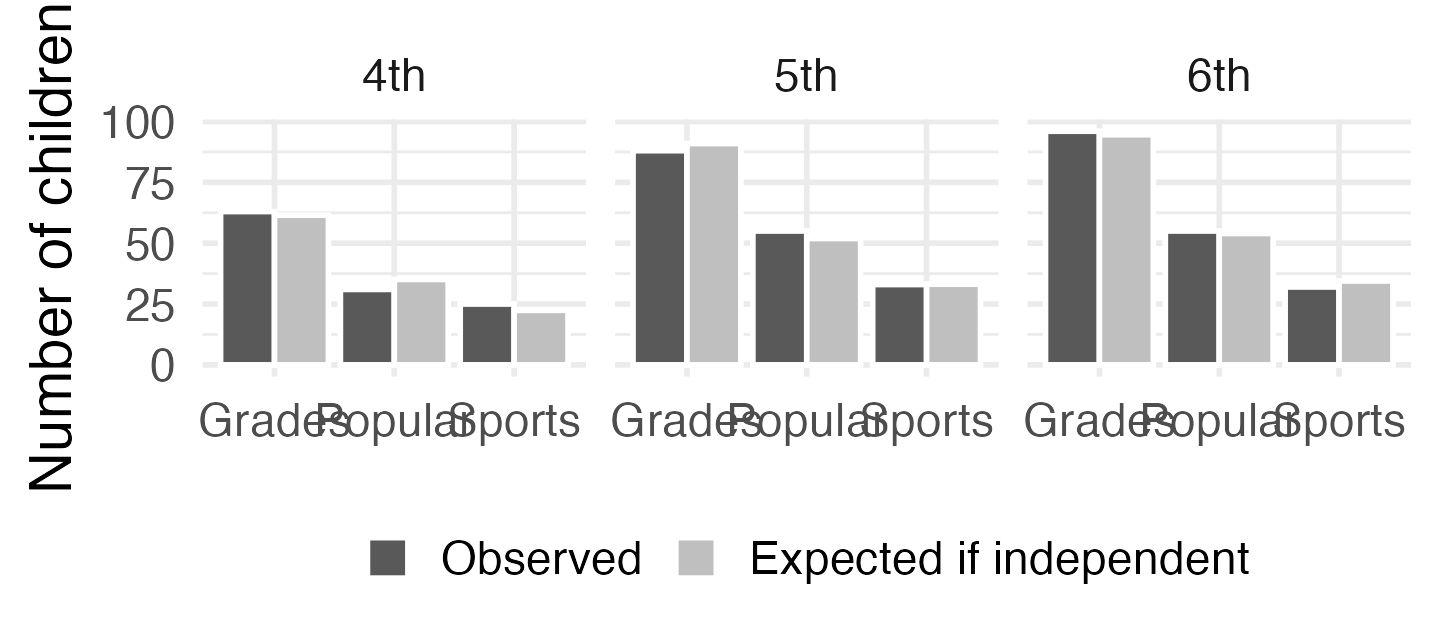
\includegraphics[width=0.9\textwidth]{popular_obs_vs_exp.png}
\end{center}

\vspace{-0.4em}
Every cell is close to what independence predicts. But ``close'' is a judgment, and different people will judge differently. \hl{We need to turn the whole picture into a single number, and then ask how unusual that number is.}

\end{frame}

%%%%%%%%%%%%%%%%%%%%%%%%%%%%%%%%%%%%%%%%%%%%%%%%%%%%%%%%%%%%%%%%%%%%%%%%
\section{One number for the whole table}
%%%%%%%%%%%%%%%%%%%%%%%%%%%%%%%%%%%%%%%%%%%%%%%%%%%%%%%%%%%%%%%%%%%%%%%%
\begin{frame}
\frametitle{The chi-square statistic}

\formula{$X^2$: the distance between the table and independence}{
\[
X^2 \;=\; \sum_{\text{all cells}} \frac{(O - E)^2}{E}
\]
where $O$ is the observed count in a cell and $E$ the expected count under independence.}

\vspace{0.1em}
{\footnotesize
\begin{itemize}
\item \hl{Squared}, so a cell $5$ above and a cell $5$ below do not cancel out.
\item \hl{Divided by $E$}: being $5$ off matters far more where we expect $10$ than where we expect $1000$.
\item $X^2 = 0$ means a table matching independence exactly. It only grows from there.
\end{itemize}}

\end{frame}

%%%%%%%%%%%%%%%%%%%%%%%%%%%%%%%%%%%%%%%%%%%%%%%%%%%%%%%%%%%%%%%%%%%%%%%%
\begin{frame}
\frametitle{Computing it for the schoolchildren}

Nine cells, each contributing $(O-E)^2/E$:
\[
\frac{(63 - 61.5)^2}{61.5} + \frac{(31 - 35.1)^2}{35.1} + \cdots + \frac{(32 - 34.5)^2}{34.5}
\;=\; \hl{$X^2_{\mathrm{obs}} = 1.312$} .
\]
\vspace{0.3em}
\dq{Is $1.312$ big or small? \emph{What would you need to know} to answer that, and how would you get it?}

\pause
\vspace{-0.2em}
\solnbox{\small A statistic means nothing on its own. We need the \hl{null distribution of $X^2$}: how it behaves in tables where the two variables really are independent. We have two ways to get one.}

\end{frame}

%%%%%%%%%%%%%%%%%%%%%%%%%%%%%%%%%%%%%%%%%%%%%%%%%%%%%%%%%%%%%%%%%%%%%%%%
\section{Two roads to the null distribution}
%%%%%%%%%%%%%%%%%%%%%%%%%%%%%%%%%%%%%%%%%%%%%%%%%%%%%%%%%%%%%%%%%%%%%%%%
\begin{frame}
\frametitle{Road A: shuffle the labels}

\keyidea[-- exchangeability]{If grade and goal really are independent, then a child's answer had nothing to do with their grade, so that answer could equally well have belonged to \emph{any} of the $478$ children. The goal labels are \hl{exchangeable}.}

\vspace{0.3em}
So we impose $H_0$ by brute force:

\vspace{-0.2em}
{\small
\begin{enumerate}
\item Keep the $478$ grades as they are; \hl{shuffle} the $478$ goals among them.
\item Rebuild the table and recompute $X^2$.
\item Repeat $10{,}000$ times. That is the null distribution.
\end{enumerate}}

\vspace{0.2em}
{\small The row and column totals never change. Only which child holds which label.}

\end{frame}

%%%%%%%%%%%%%%%%%%%%%%%%%%%%%%%%%%%%%%%%%%%%%%%%%%%%%%%%%%%%%%%%%%%%%%%%
\begin{frame}
\frametitle{What one shuffle actually does}

\vspace{-0.2em}
\begin{center}
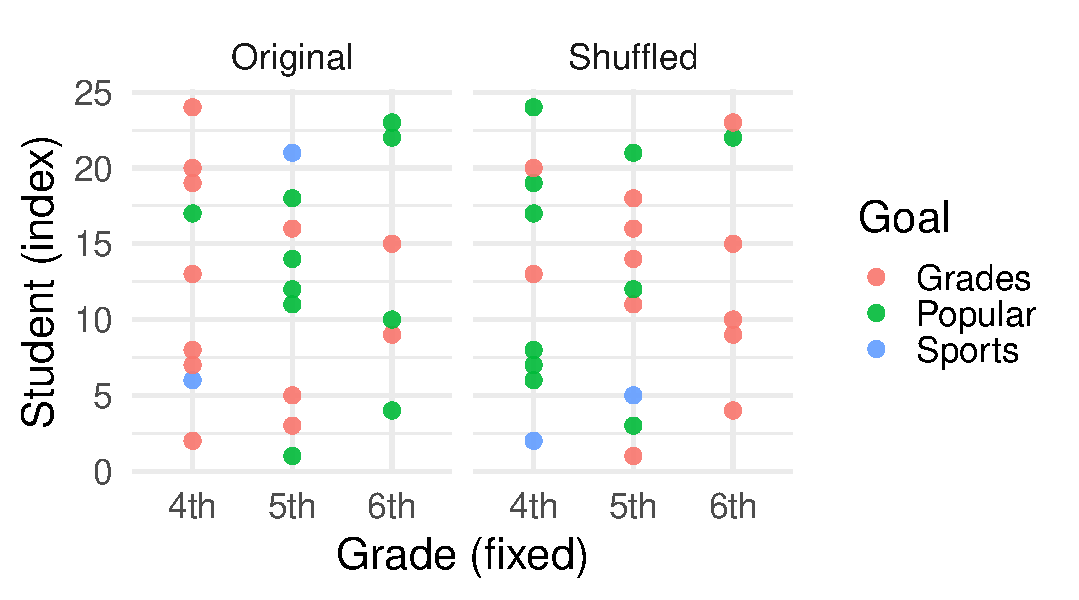
\includegraphics[width=0.78\textwidth]{popular_perm_step.pdf}
\end{center}

\vspace{-0.5em}
{\small The same $478$ children stand in the same grades. Only the \emph{goal} labels have been dealt out again at random, which is precisely the world $H_0$ describes. Do this $10{,}000$ times and you have the null distribution.}

\end{frame}

%%%%%%%%%%%%%%%%%%%%%%%%%%%%%%%%%%%%%%%%%%%%%%%%%%%%%%%%%%%%%%%%%%%%%%%%
\begin{frame}[fragile]
\frametitle{Road A in R}

\begin{lstlisting}[language=R, basicstyle=\ttfamily\scriptsize]
# kids: one row per child, columns grade and goal
x2_of <- function(a, b) {          # X^2 of any two columns
  O <- table(a, b)
  E <- outer(rowSums(O), colSums(O)) / sum(O)
  sum((O - E)^2 / E)
}

x2_obs <- x2_of(kids$grade, kids$goal)        # 1.312

null <- replicate(10000,
  x2_of(kids$grade, sample(kids$goal)))       # shuffle!

mean(null >= x2_obs)                          #> 0.866
\end{lstlisting}

\vspace{-0.3em}
{\small The p-value is one-sided by construction: only \emph{large} $X^2$ is evidence against independence, because $X^2$ cannot go below zero.}

\end{frame}

%%%%%%%%%%%%%%%%%%%%%%%%%%%%%%%%%%%%%%%%%%%%%%%%%%%%%%%%%%%%%%%%%%%%%%%%
\begin{frame}
\frametitle{Road B: a formula for the null distribution}

A statistic that is a mean has a known null distribution, the normal. Here $X^2_{\mathrm{obs}}$ is the one number from our table, and we judge it against a reference distribution, $\chi^2_{df}$.

\vspace{0.2em}
\formula{The chi-square model}{
If $H_0$ holds and the expected counts are large enough,
\[
X^2 \;\approx\; \chi^2_{df},
\qquad
df \;=\; (\#\text{rows} - 1)\times(\#\text{columns} - 1) .
\]}

\vspace{0.1em}
{\small The \hl{$\chi^2_{df}$ distribution} is a new shape: it lives on $[0,\infty)$ (a squared distance cannot be negative), it is right-skewed, and its \emph{mean is exactly $df$}. One parameter, and $df$ is it.}

\end{frame}

%%%%%%%%%%%%%%%%%%%%%%%%%%%%%%%%%%%%%%%%%%%%%%%%%%%%%%%%%%%%%%%%%%%%%%%%
\begin{frame}
\frametitle{Why $df = 4$, and not $9$?}

Nine cells, but \hl{the row and column totals are fixed}. They are what we conditioned on to get the expected counts, so most cells cannot move freely.

\vspace{0.1em}
\begin{center}
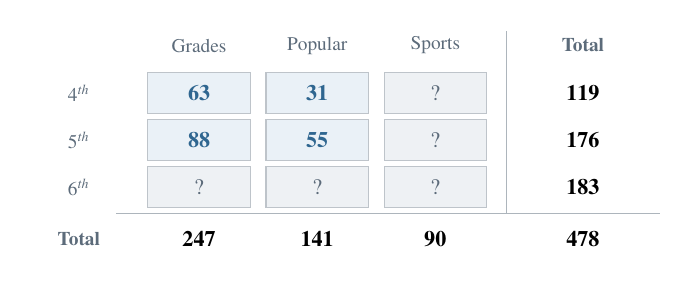
\begin{tikzpicture}[
  x=1.5cm, y=0.60cm, font=\footnotesize,
  cell/.style   ={minimum width=1.3cm, minimum height=0.52cm, draw=ccGray!40},
  free/.style   ={cell, fill=ccBlueBg, text=ccBlue, font=\footnotesize\bfseries},
  forced/.style ={cell, fill=ccGrayBg, text=ccGray},
  tot/.style    ={minimum width=1.3cm, minimum height=0.52cm, font=\footnotesize\bfseries},
  hdr/.style    ={minimum width=1.3cm, font=\scriptsize, text=ccGray}]
  \node[hdr] at (1,1) {Grades};  \node[hdr] at (2,1) {Popular};
  \node[hdr] at (3,1) {Sports};  \node[hdr] at (4.25,1) {\textbf{Total}};
  \node[hdr, anchor=east] at (0.42,0)  {$4^{th}$};
  \node[hdr, anchor=east] at (0.42,-1) {$5^{th}$};
  \node[hdr, anchor=east] at (0.42,-2) {$6^{th}$};
  \node[hdr, anchor=east] at (0.42,-3.1) {\textbf{Total}};
  \node[free] at (1,0)  {63}; \node[free] at (2,0)  {31}; \node[forced] at (3,0)  {?};
  \node[free] at (1,-1) {88}; \node[free] at (2,-1) {55}; \node[forced] at (3,-1) {?};
  \node[forced] at (1,-2) {?}; \node[forced] at (2,-2) {?}; \node[forced] at (3,-2) {?};
  \node[tot] at (4.25,0) {119}; \node[tot] at (4.25,-1) {176}; \node[tot] at (4.25,-2) {183};
  \node[tot] at (1,-3.1) {247}; \node[tot] at (2,-3.1) {141}; \node[tot] at (3,-3.1) {90};
  \node[tot] at (4.25,-3.1) {478};
  \draw[ccGray!50] (0.3,-2.55) -- (4.9,-2.55);
  \draw[ccGray!50] (3.6,1.3) -- (3.6,-2.55);
\end{tikzpicture}
\end{center}

\vspace{-0.1em}
{\small Choose the \hl{four} blue cells freely and the other five are forced. $df=(3-1)\times(3-1)=4$ counts exactly that.}

\end{frame}

%%%%%%%%%%%%%%%%%%%%%%%%%%%%%%%%%%%%%%%%%%%%%%%%%%%%%%%%%%%%%%%%%%%%%%%%
\begin{frame}
\frametitle{And the two roads agree}

\vspace{-0.3em}
\begin{center}
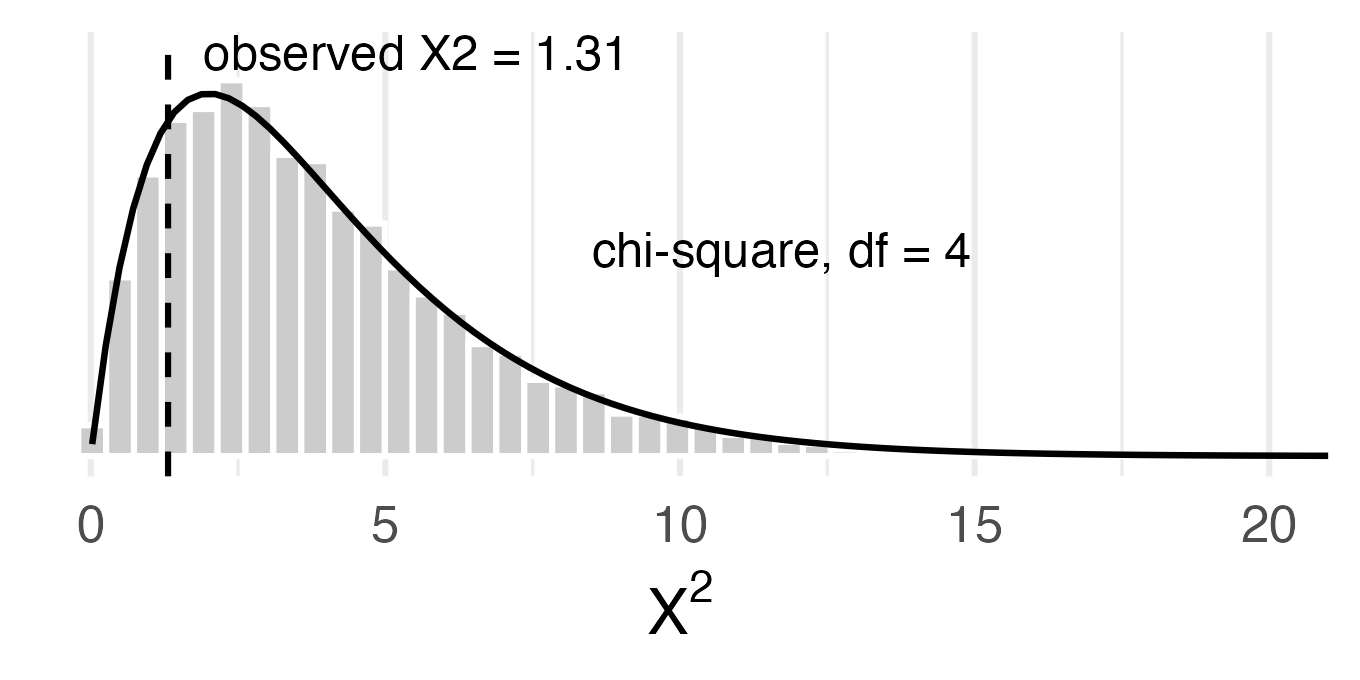
\includegraphics[width=0.68\textwidth]{chisq_vs_shuffle.png}
\end{center}

\vspace{-0.5em}
\keyidea{Shuffling gave $p = 0.866$, the formula $p = 0.859$. The mean of the $10{,}000$ shuffled $X^2$ values was $3.98$, and a $\chi^2_{4}$ distribution has mean exactly $4$. Nobody arranged that.}

\end{frame}

%%%%%%%%%%%%%%%%%%%%%%%%%%%%%%%%%%%%%%%%%%%%%%%%%%%%%%%%%%%%%%%%%%%%%%%%
\begin{frame}
\frametitle{When may I use the formula?}

\begin{itemize}
\item \hl{Independent observations}: one row of the table per child, and no child counted twice.
\item \hl{Every expected count at least 5.} Here the smallest is $22.4$, so we are comfortable.
\end{itemize}

\vspace{0.4em}
\caution{%
\begin{itemize}\setlength{\itemsep}{1pt}
\item The condition is on the \emph{expected} counts, not the observed ones.
\item On a sparse table (a rare category, a small sample) the $\chi^2$ curve fits poorly and the p-value is wrong.
\item \hl{Shuffling has no such condition:} it is valid whatever the counts.
\end{itemize}}

\end{frame}

%%%%%%%%%%%%%%%%%%%%%%%%%%%%%%%%%%%%%%%%%%%%%%%%%%%%%%%%%%%%%%%%%%%%%%%%
\begin{frame}
\frametitle{Does that condition actually matter?}

\vspace{-0.2em}
\begin{center}
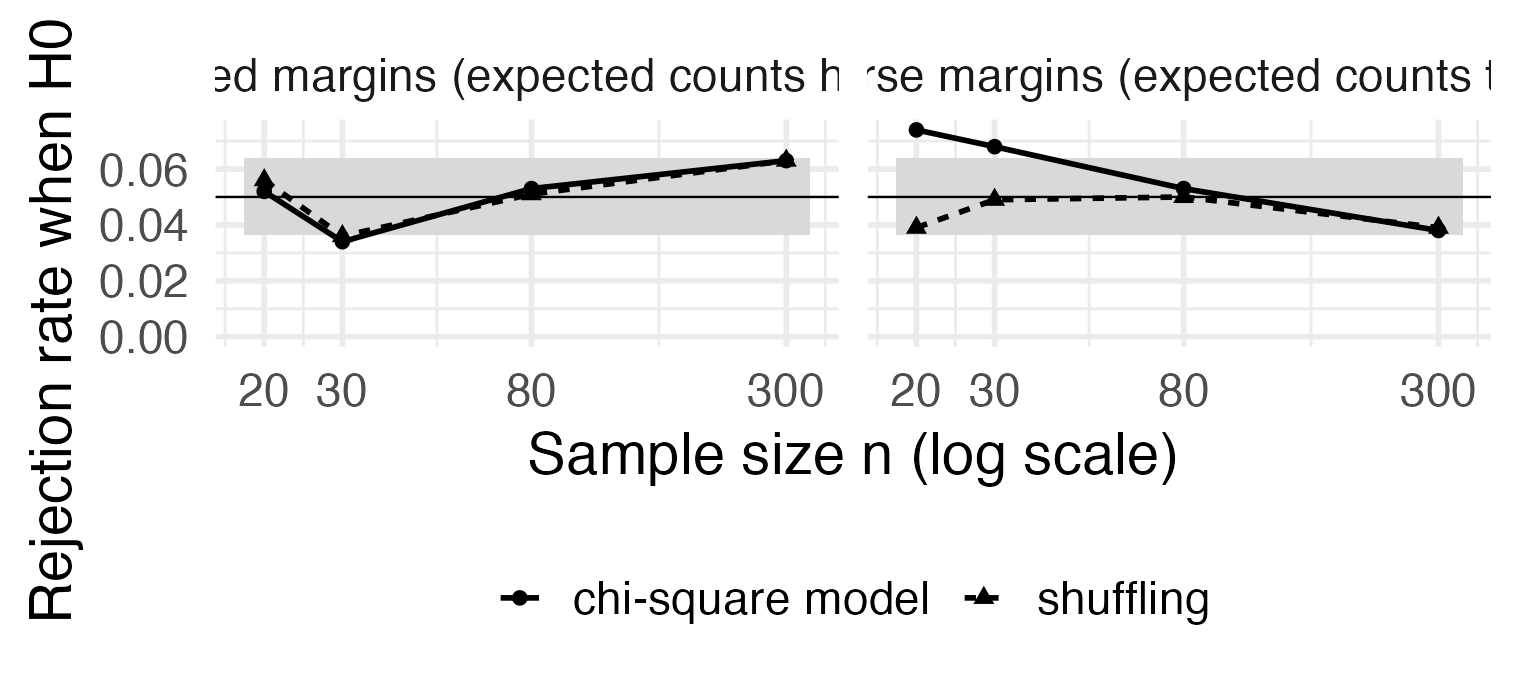
\includegraphics[width=0.82\textwidth]{chisq_condition_check.png}
\end{center}

\vspace{-0.5em}
{\footnotesize
\begin{itemize}\setlength{\itemsep}{1pt}
\item $1{,}000$ tables in which the two variables really \emph{were} independent.
\item A working test should reject $H_0$ $5\%$ of the time.
\item \hl{On sparse tables with small $n$ the chi-square model rejects $7$--$8\%$}, finding associations that are not there.
\item Shuffling stays at $5\%$ throughout.
\end{itemize}}

\end{frame}

%%%%%%%%%%%%%%%%%%%%%%%%%%%%%%%%%%%%%%%%%%%%%%%%%%%%%%%%%%%%%%%%%%%%%%%%
\begin{frame}
\frametitle{So: do goals vary by grade?}

\vspace{-0.2em}
\[
X^2 = 1.31 \;\text{ on } 4 \text{ df}, \qquad p = 0.86 .
\]
\vspace{-0.3em}
{\small If grade and goal were unrelated, a table at least this far from independence would turn up about \textbf{86\% of the time}. Ours is unremarkable. \hl{No evidence that what children care about varies by grade.}}

\vspace{0.2em}
\caution{That is \emph{not} ``we have shown they are independent''. $p = 0.86$ means the data are \emph{consistent} with independence. We have no evidence against it. \emph{Absence of evidence is not evidence of absence} (Lecture 8).}

\end{frame}

%%%%%%%%%%%%%%%%%%%%%%%%%%%%%%%%%%%%%%%%%%%%%%%%%%%%%%%%%%%%%%%%%%%%%%%%
\section{What a real dependence looks like}
%%%%%%%%%%%%%%%%%%%%%%%%%%%%%%%%%%%%%%%%%%%%%%%%%%%%%%%%%%%%%%%%%%%%%%%%
\begin{frame}
\frametitle{Activity: the Portal exclosure experiment}

Some plots at the Portal site are ringed by fences with gaps too small for a \hl{kangaroo rat}. Others are open controls. Every rodent caught was recorded, for decades.

\vspace{0.1em}
{\scriptsize
\begin{center}
\begin{tabular}{lrrrrr}
\toprule
Captures & Control & Long-term & Rodent & Short-term & Spectab \\
& & Krat excl. & excl. & Krat excl. & excl. \\
\midrule
\textbf{DM} (kangaroo rat) & 6760 & 245 & 851 & 1156 & 1584 \\
\textbf{DS} (kangaroo rat) & 1389 & 26 & 104 & 465 & 520 \\
\textbf{PP} (pocket mouse) & 1108 & 879 & 241 & 573 & 322 \\
\bottomrule
\end{tabular}
\end{center}}

\vspace{-0.1em}
\app{Before computing: is species independent of plot type? Which cells should sit furthest from independence, and in which direction?}

\end{frame}

%%%%%%%%%%%%%%%%%%%%%%%%%%%%%%%%%%%%%%%%%%%%%%%%%%%%%%%%%%%%%%%%%%%%%%%%
\begin{frame}
\frametitle{Activity: the Portal exclosures --- the verdict}
\examplehead{Portal exclosures}

{\small The smallest expected count is $177.5$, so the $\chi^2$ model is safe here.}
\vspace{-0.4em}
\[
X^2 = 3062 \;\text{ on } 8 \text{ df}, \qquad p < 2\times 10^{-16} .
\]
\vspace{-0.3em}
\solnbox{\small Overwhelming evidence that species and plot type are \emph{not} independent, which is exactly what a fence is \emph{for}. And because this is a designed experiment rather than an observational table, we may even call the dependence causal.}

\vspace{0.2em}
{\small \hl{But which cells depart from independence?} Compressing fifteen numbers into one $X^2$ loses that detail.}

\end{frame}

%%%%%%%%%%%%%%%%%%%%%%%%%%%%%%%%%%%%%%%%%%%%%%%%%%%%%%%%%%%%%%%%%%%%%%%%
\begin{frame}
\frametitle{Standardized residuals: the pieces $X^2$ is built from}
\examplehead{Portal exclosures}

\formula{Standardized residual: observed count $O$, expected count $E$}{
\[
\frac{O - E}{\sqrt{E}} \qquad \text{(in standard errors)}
\]}

\vspace{-0.3em}
\begin{center}
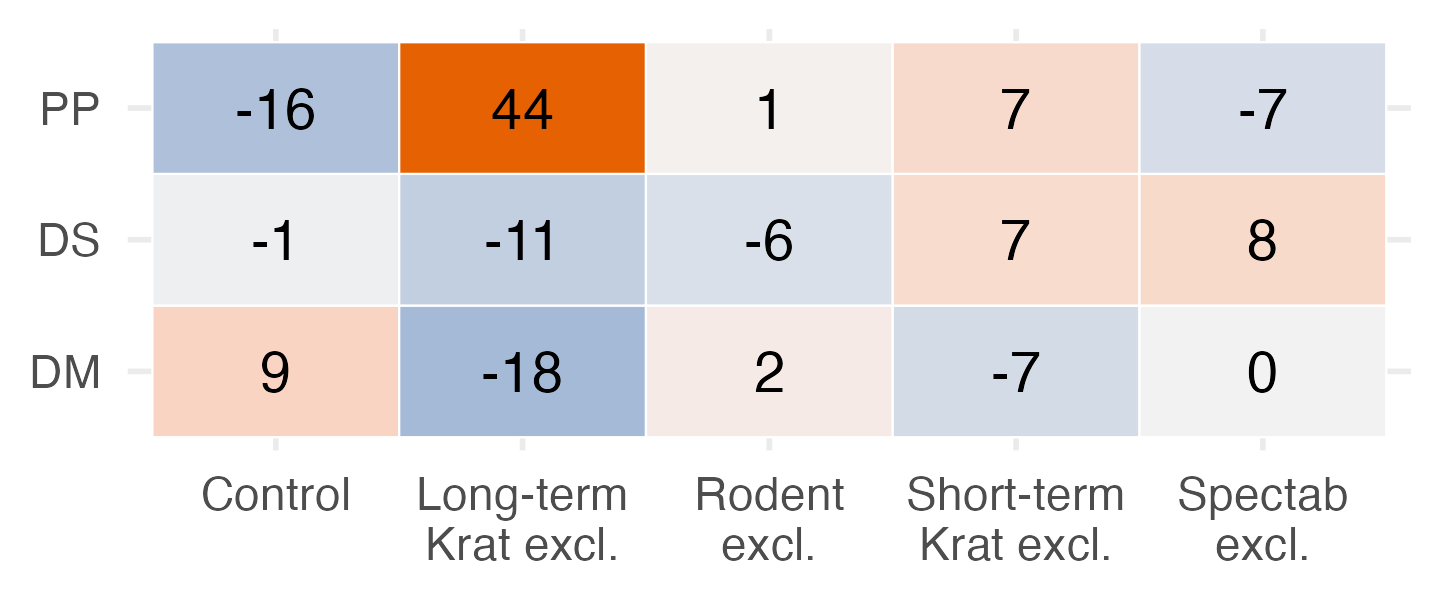
\includegraphics[width=0.74\textwidth]{portal_residuals.png}
\end{center}

\end{frame}

%%%%%%%%%%%%%%%%%%%%%%%%%%%%%%%%%%%%%%%%%%%%%%%%%%%%%%%%%%%%%%%%%%%%%%%%
\begin{frame}
\frametitle{Read the residuals, not just the p-value}
\examplehead{Portal exclosures}

\keyidea[-- the ecology falls out of the table]{The biggest cell is not a kangaroo rat. In the long-term kangaroo-rat exclosure the \emph{pocket mouse} sits at $+44$: remove the competitor, and another species takes over. The p-value establishes \emph{that} something happened. The residuals show \emph{what}.}

\vspace{0.5em}
\caution{$X^2$ is an \emph{omnibus} test: a large value never identifies which cells are responsible. Look at the residuals before you write the sentence.}

\end{frame}

%%%%%%%%%%%%%%%%%%%%%%%%%%%%%%%%%%%%%%%%%%%%%%%%%%%%%%%%%%%%%%%%%%%%%%%%
\section{Wrap-up}
%%%%%%%%%%%%%%%%%%%%%%%%%%%%%%%%%%%%%%%%%%%%%%%%%%%%%%%%%%%%%%%%%%%%%%%%
\begin{frame}
\frametitle{Two roads, whatever the statistic}

{\scriptsize
\begin{center}
\setlength{\tabcolsep}{4pt}
\begin{tabular}{lll}
\toprule
\textbf{The statistic} & \textbf{By simulation} & \textbf{By formula} \\
\midrule
a proportion & simulate $H_0$ (Lec 8) & binomial, exact; $z$ (Lec 10) \\
a mean or a difference & bootstrap (Lec 9), permute (Lec 8) & the CLT: $z$, $t$ (Lec 10) \\
\hl{a whole table, $X^2$} & \hl{permute one column (today)} & \hl{$\chi^2_{df}$ (today)} \\
\bottomrule
\end{tabular}
\end{center}}

\vspace{0.2em}
The recipe never changes: \emph{state $H_0$, build a statistic, get its null distribution (by simulating $H_0$, or by a formula whose conditions hold), then count how extreme the observed value is.}

\vspace{0.1em}
{\small Only the statistic, and the formula that fits it, change.}

\end{frame}

%%%%%%%%%%%%%%%%%%%%%%%%%%%%%%%%%%%%%%%%%%%%%%%%%%%%%%%%%%%%%%%%%%%%%%%%
\begin{frame}
\frametitle{Summary}

\begin{itemize}
\item A \hl{two-way table} cross-classifies two categorical variables. $H_0$ is that they are \hl{independent}.
\item Independence makes a prediction: the \hl{expected counts} $E_{ij} = (\text{row}_i)(\text{col}_j)/n$.
\item \hl{$X^2 = \sum (O-E)^2/E$} compresses the whole table into one distance-from-independence.
\item Its null distribution comes either from \hl{shuffling} one variable (always valid) or from the \hl{$\chi^2_{df}$ model} with $df = (r-1)(c-1)$ (valid when every expected count is at least 5).
\item A large $X^2$ says the table is not independent; the \hl{standardized residuals} say \emph{where}.
\end{itemize}

\end{frame}

%%%%%%%%%%%%%%%%%%%%%%%%%%%%%%%%%%%%%%%%%%%%%%%%%%%%%%%%%%%%%%%%%%%%%%%%
\begin{frame}
\frametitle{Coming up next}

\hl{Next class, analysis of variance:} what if there are \emph{three or more} groups of numbers? Do four fertilizers give different mean yields?

\begin{itemize}
\item why running all the pairwise $t$-tests is a trap;
\item comparing variability \emph{between} groups with variability \emph{within} them;
\item the same two roads: shuffle the group labels, or use a mathematical model. This one is called the \hl{$F$ distribution}.
\end{itemize}

\end{frame}

%%%%%%%%%%%%%%%%%%%%%%%%%%%%%%%%%%%%%%%%%%%%%%%%%%%%%%%%%%%%%%%%%%%%%%%%

%%%%%%%%%%%%%%%%%%%%%%%%%%%%%%%%%%%%
% End document
%%%%%%%%%%%%%%%%%%%%%%%%%%%%%%%%%%%%

\end{document}
